
\chapter{Investigating the emergence of communication systems}

One of the most important findings of cognitive science has been the
insight that even supposedly simple mental tasks such as recognizing
objects or performing arm movements are actually the result of a
complex interplay between a highly interwoven network of cognitive
processes, the body, and the physical world and the social
environment. And it turned out that the capability to use symbolic
language -- one of the few features (if not the only) that sets us
apart from the animal kingdom -- is not an isolated mental skill
either but relies on and emerges from large parts of the cognitive
apparatus that is available to us. Progress in neuroscience and
related areas has given us quite some understanding of the underlying
mechanisms of perception, motor control, memory, etc., but theories of
``how language works'' are just beginning to emerge.

Coming from an artificial intelligence background, we want to explore
the question of ``how language could work'' by designing artificial
robotic agents that learn to communicate with each other about things
in their environment. This involves finding solutions to a wide
variety of challenges: how can we build robots that are able to
perceive the world, that construct persistent mental representations
of what they experience, that interact socially with each other and --
most importantly -- that have the capability to communicate? Endowing
our agents with a ``capability to communicate'' does not mean that we
will give them a pre-existing language. We will instead investigate
how they can self-organize communication systems through local
conversations, i.e. how they can agree on a shared language in order
to communicate successfully. 

The work presented in this thesis will not cover the whole complexity
of human language (which would include grammar, morphology, etc.) but
we will focus on lexicon formation. That means we will show how agents
can learn names for objects in their environment (i.e. words similar
to proper names such as ``John'', adjectives such as ``green'' and
nouns such as ``block'') from each other. We will start from very
simple models and then demonstrate how the increased complexity of
communicative challenges and agent architectures leads to more complex
word learning models. In series of controlled experiments we will
evaluate the performance of these models as well as the influence of
internal and external factors -- both in simulated environments where
agents have idealized abstract perceptions of the world and with
actual physical robots, which will allow us to analyse the impact of
embodiment on the dynamics of the interactions.


\begin{figure}[t]
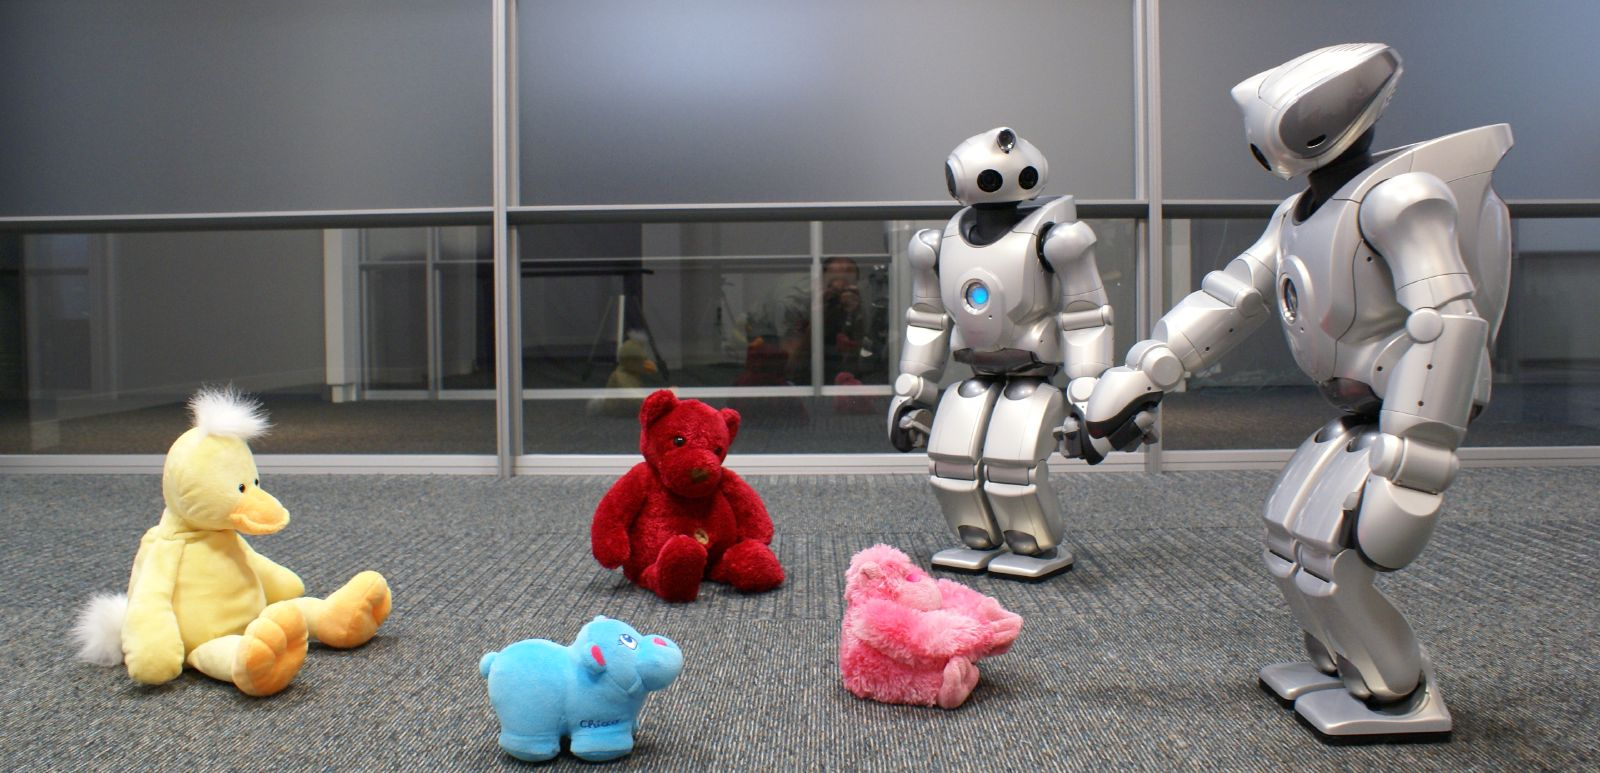
\includegraphics[width=\textwidth]{figures/photo-2-qrios-with-4-toys}
\caption{Example of a communicative interaction between two
  agents. The robots perceive objects in their shared environment
  through their built-in cameras and subsequently engage in a
  conversation about one of the objects. Over the course of repeated
  such interactions, populations of agents are able to coordinate
  their conceptual repertoires for recognizing and classifying objects
  as well as a shared language for communicating about them.}
\label{f:photo-2-qrios-with-4-toys}
\end{figure}

Let us give an example of how such an experiment could look
like. Figure \ref{f:photo-2-qrios-with-4-toys} shows two robotic
agents that are placed in an office environment with a set of toy
objects in front of them. The robot at the right will take the role of
the speaker and the other the role of a hearer. The communicative goal
of the speaker will be to draw the attention of the hearer to one of
the objects (e.g. the pink monkey). For this, he will first have to
classify the visual experience of the object with respect to how
similar it is to mental representations of previously experienced
objects (i.e. he has to recognize the pink monkey as a {\tt monkey},
as something {\tt pink}, as {\tt the closest object}, etc.) -- or, in
case he has never before seen a similar looking object, construct such
a representation. Then, the speaker will use words from his own
private linguistic inventory that he associates with the recognized
concepts and that he thinks of will serve his communicative goal best
(and again invent words when he does not know how to express the
concepts). The hearer will then try to interpret the utterance using
his own sensory experience of the scene and his own private conceptual
and linguistic repertoires. The hearer infers the communicative goal
of the speaker by finding the object that fits best the concepts
associated to the words heard. It can of course happen that both
agents connect different meanings to the words of the utterance. To
avoid potential misunderstandings, the hearer points to the object
that he understood and the speaker will either signal a confirmation
(if the object pointed at was indeed the one he intended) or otherwise
point to the correct object. It might furthermore happen that the
hearer does not know one of the words at all or is otherwise not able
to infer the topic of the conversation -- also in this case the
speaker will point to the object he had in mind, allowing the hearer
to learn the meaning of the word.



For taking part in such interactions, the robots certainly need to be
endowed with a powerful set of mental capabilities and we will analyze
what these have to be. Building robotic systems that are able to
self-organize linguistic communication systems from scratch is a very
exciting -- and also extraordinarily difficult -- engineering
challenge. It involves dealing with high levels of complexity in the
interaction of the different cognitive processes and we will explore
how (by going from simple models to more advanced ones) the complexity
of different dynamics can be handled and explained. In addition to
that, we will take inspiration from psychologists and linguists such
as
\cite{tomasello03constructing,tomasello99cultural,tomasello08origins,bloom00how-children,bowerman01language}
who discuss human intelligence and language as a result of
capabilities for engaging in social activities, for constructing
mental representations about the world and other general learning
mechanisms. We will demonstrate how their theories about language and
cognition can be operationalized in computational models and
additionally use these models to verify hypotheses coming out of these
research fields. In this chapter we will lay out the theoretical
foundations for this work. Chapter \ref{c:building-blocks} will
introduce the methods and tools that were used for our experiments and
then Chapter \ref{c:thesis-overview} will sum up this introduction by
giving an overview of the work.\\

\noindent This thesis' investigations are a truly multidisciplinary endeavour:
we will borrow ideas from artificial intelligence, robotics, 
psychology, linguistics and philosophy and -- although our
contribution is clearly rooted in artificial intelligence -- we also
want to be relevant to all of these disciplines. Before we begin, let
us set the stage by outlining the theoretical and methodological basis
for our experiments as well as embed the work in the literature (those
readers who are familiar with the research field of artificial
language evolution can safely skip this part and continue with Chapter
\ref{c:building-blocks}).



\section{Basic assumptions}
\label{s:basic-assumptions}

The question of what language is, how it is learnt, how it changes,
which cognitive mechanisms are involved, etc. (in short: how it works)
is far from being settled -- in fact, the study of language is
probably the field within the cognitive sciences with the biggest
variety of competing theories. Many ideas that were considered to be
state of the art in the recent past are nowadays seen as outdated by
younger scholars but still receive attention and support by major
parts of the scientific community. Due to this absence of a common
theoretical basis, it is very likely that the particular view on
language taken in thesis is not shared by many linguists,
psychologists and philosophers. However, defending this view against
competing theories would be beyond the scope of this thesis. Instead,
we explicitly enumerate our basic assumptions and then go on from
there -- we'll leave the discussion of these premises to the
referenced literature.

Additionally, we will discuss the empirical methods chosen for our
experiments. Trying to answer questions about language and cognition
by building and running computational models is a rather new approach
and scientific standards still have to be agreed upon. Over their long
history, related disciplines have established a set of principles and
rules of what can be considered a valid contribution to their fields:
insights are either gained by conducting carefully controlled
experiments with human subjects (with the methods for experiment
design and data interpretation well defined) or by systematically
analyzing human languages. With the subjects of the investigations
here being computer programs embodied in robots and emerging
artificial communication systems, the methods of psychology and
linguistics can't be applied and the question is how results of our
research can be a contribution to the understanding of human
language. Furthermore, even within the modeling community there is
only little consensus of how to do experiments and how to reach
progress (and there are many examples with poor scientific
quality). It is thus understandable that many psychologists and
linguistics hesitate to accept results from modeling work. But since
we want to use computational modeling for understanding how language
works and furthermore want the work to be relevant to people outside
of artificial intelligence, a thorough and consistent methodology
needs to be followed.


\subsection{Communication and language acquisition as a social act}
\label{s:communication-as-a-social-act}

Communication is commonly understood (by computer scientists, but also
many others) as a process in which a sender sends information to a
receiver. Information is encoded into a message and transmitted over a
medium to the receiver, which then decodes the message again. When for
example a speaker says ``the dog is hungry'' the information that the
dog is hungry (e.g. {\tt dog(x)}$\wedge$ {\tt hungry(x)}) is encoded
into an English sentence. The hearer is able to decode the sentence
because he speaks the same language, i.e. he uses the same rules to
produce and interpret utterances. 

However, uttering a sentence such as above is something else than sole
transmission of information. According to \cite{tomasello99cultural},
it is part of a co-operative activity that both speaker and hearer are
involved in: built on a \emph{common ground} (the interlocutors'
mutual understanding of each others knowledge and goals,
\citealp{clark91grounding}), speaking is an action in which the
speaker attempts to affect the mental states of the hearer -- usually
by drawing the attention of the listener to something in the world
(e.g. an object, an event, a property of an object etc.). Uttering the
sentence ``the dog is hungry'' is an action that could have several
communicative goals (depending on their shared environment and
previous discourse): the speaker could want his child to feed the dog,
he could want a stranger to leave his property, or warn a friend of a
potentially dangerous animal. The speaker does not say all this -- he
implicitly assumes that the hearer will infer the communicative
intention and perform the desired action.\\


\noindent Where does then the human capacity for performing communicative acts
and interpreting them come from and how do children learn the language
of their parents? In the \emph{nativist view}
\citep*{chomsky57syntactic-structures,pinker90natural,hauser02faculty},
language development is seen as the result of genetically predefined
abilities that are independent from the development of other
skills. All humans are born with an innate ``language organ'' (the
\emph{language acquisition device}) and learning the language of a
particular culture means adapting parameters of an ``universal
grammar''. Although the nativist view occupied generations of
linguists and although it is probably still one of the most widespread
theories around, we find its assumptions so fallacious and unnatural
that we will not discuss it here -- for a review of arguments against
nativism refer e.g. to \cite{tomasello05beyond} and to the majority of
the other theoretical literature listed in our references
(e.g. \citealp{steels03evolution}).

\cite{piaget52origins} saw the non-social interaction with the
environment as the main source of language development: because
parents usually make sure that a rabbit is in the field of view of a
child when they say the word ``rabbit'', children can passively learn
the associations between words and their meanings in a similar way as
they learn other facts about the external world. In this tradition,
the \emph{constraints} approach (e.g.
\citealp{markman92constraints,gleitman90structural}) proposes
(possibly innate) learning mechanisms (i.e. constraints) that enable
the child to \emph{map} what it hears to what it sees. But ``learning
a word is a social act. When children learn that rabbits eat carrots,
they are learning something about the external world, but when they
learn that \emph{rabbit} refers to rabbits, they are learning an
arbitrary convention shared by a community of speakers, an implicitly
agreed-upon way of communicating'' \citep[p. 55]{bloom00how-children}.

We will hence adopt the \emph{social-pragmatic view} in this thesis:
``In the social-pragmatic view, young children are not engaged in a
reflective cognitive task in which they are attempting to make correct
mappings of word to world based on adult input, but rather they are
engaged in social interactions in which they are attempting to
understand and interpret adult communicative intentions -- so as to
make sense of the current situation''
\citep[p. 135]{tomasello01perceiving}. The major cognitive skill
involved in language learning is thus not a set of learning
constraints but ``their understanding that other persons have
intentions towards their intentional states''
\citep[p. 135]{tomasello01perceiving}. So when a child hears the word
``rabbit'', it learns the meaning of this word not because she sees a
rabbit, but because she can interpret the communicative intentions of
the adult. In addition to the ability to engage in communicative
interactions, to establish shared attention and to culturally learn
from such interactions, language learning requires an ``\dots unique
motivation to share psychological states with others and unique forms
of cognitive representation for doing so''
\citep*[p. 675]{tomasello05understanding} -- humans are thus
intrinsically motivated to engage in collaborative interactions and to
cooperate.

Consequently, language learning does not rely on a specific
\emph{language acquisition device}, but on skills that evolved and
developed for other purposes: the ability to infer the intentions of
others, the ability to acquire concepts, and certain general learning
and memory capabilities.



\subsection{Language as a complex adaptive system}
\label{s:language-as-a-complex-adaptive-system}

A language is not a self-contained body of fixed rules that are
internalized by everybody who speaks the language (as it is the case
in many engineered communication systems in computer science), but it
is a set of conventions shared by a community of language users. What
words mean and how they are to be combined into proper sentences
according to the grammar of a language is not dictated by authorities
or institutions such as for example dictionary publishers. Instead,
each single convention is established and adapted through ongoing
linguistic behavior (conversations). New words, phrases and
grammatical constructions continuously enter a language, word meanings
can change over time and expressions can even disappear from a
language (see
e.g. \citealp{croft00explaining,deutscher05unfolding}). Language
learning and language change happens in local dialogues between
speakers of the language in order to adapt to changing communicative
needs (e.g. when new artifacts or knowledge enter a culture), as a
result of contact with other language communities or to improve
expressiveness in general.

This has lead researchers to conceptualize language as a \emph{complex
  adaptive system} \citep{steels00language} and investigate it by
means of analytical models and computer simulations. The global
phenomenon of a coherent and shared language is understood in terms of
the local interactions between language users -- in a similar way that
the properties of a gas can be analyzed as the result of the physical
interaction of molecules, the functioning of a cell as the interplay
between complex enzyme networks, or market dynamics based on models of
single economic actors (see for example
\citealp*{castellano09statistical}, for a review of how methods from
statistical physics have been applied to a big variety of social
dynamics).

The basic idea is that shared linguistic communication systems
\emph{emerge} through processes of \emph{self-organization}. Words and
grammatical constructions are mutually \emph{adopted} by agents and
consequently \emph{propagate} in the population. No agent has a
complete view over the language but each agent maintains its own set
of inventories, shaped only through local interactions with other
agents (no agent can directly control the linguistic behavior of the
whole population). A language community is an open system, i.e. new
agents can enter at any time and new communicative challenges may
arise. When existing inventories are not not adequate, agents adapt or
extend them (e.g. by inventing words or by adopting existing
linguistic items for other uses). Furthermore, there are are
selectionist \emph{feedback} relationships between the use of
linguistic entities and their success so far in communication -- words
that are consistently used to successfully reach communicative goals
are more likely to spread in the population, leading to self-organized
\emph{coherence}. \cite{oudeyer07language} thus also conceptualized
language evolution as a \emph{Darwinian process}. Finally, language
spontaneously becomes more complex, driven by the need to optimize
communicative success and handle an agent's constraints of the
physical and cognitive apparatus.

\cite{steels06semiotic} introduced the term \emph{semiotic dynamics}
for the approach of understanding language as a function of the local
behavior of agents: ``I argue that it's the study of semiotic
dynamics: the processes whereby groups of people or artificial agents
collectively invent and negotiate shared semiotic systems, which they
use for communication or information organization'' (p.~32). The
emergence of language is investigated by making precise computational
models of how agents communicate and learn from each other and by
identifying the internal and external factors involved in the
self-organization of communication systems.






\subsection{Computational models as a tool for studying language
  evolution}

Building operational models of (robotic) agents that are able to
self-organize a language (which is the main goal of the work presented
here) is in itself a very interesting and nontrivial
challenge. Finding well-working solutions to this problem is
definitely a contribution to robotics and artificial intelligence
because it shows that and how such systems can be
engineered. Furthermore, searching for the structures and algorithms
that are needed for the successful emergence of particular
communication systems in specific environments can lead to new
intuitions and insights about cognition and language -- an approach
that can be seen as ``understanding by doing'' and that is advocated
in robotics by e.g. \cite{pfeifer06how}.

Beyond that, linguistic, psychological or philosophical theories of
how certain cognitive processes can be explained and integrated using
computational modeling. Understanding a cognitive system in terms of a
running computer simulation forces a researcher to make the
assumptions of the underlying theory explicit enough so that it can be
expressed fully in a formal programming language. Successfully running
the simulation can be seen as an existence proof that the assumed
mechanisms in principle yield similar results compared to phenomena
observed in human language. Additionally, computational models serve
as illustrations of theories because they clearly depict how certain
proposed mechanisms can function together.

The method of building artificial systems in order to understand
nature feels very natural for researchers in artificial intelligence
and robotics (since building systems is what they anyway do). However,
psychologists and linguists (who submit themselves to rigorous
scientific procedures based on controlled experiments with human
subjects) are often reluctant to accept such work as contributions to
their fields due to difficulties in judging the results: First, it is
often not clear why one particular computational model and not another
one should be the correct explanation of a real-world
phenomenon. Second, operationalizing hypothesized cognitive mechanisms
into structures and algorithms requires simplifications and the
question is how the results from such simplified models can be
generalized to human language and cognition. Third, computer modeling
experiments are often not described in enough detail so that they
could be understood and repeated by other researchers.

Acknowledging the need for more careful experimentation standards in
order to be relevant for researchers outside of computer science,
scholars such as
\cite{steels06how,cangelosi02computer,schlesinger01agent-based}
started defining sets of criteria for how to do computer simulations
in the field of artificial language evolution in a scientific
way. These efforts are still in the beginning but it seems that the
modeling community started paying more attention to the concerns
mentioned above in the recent years. Two types of questions are
usually asked in language evolution related computer modeling work:
First, how can we explain the emergence of a complex natural language
like communication system? And second, which out of two (or more)
competing linguistic theories receive the most support from a computer
simulation?

The first kind of experiments searches for the cognitive mechanisms
and external factors that are required for the successful development
of a particular communication system or for another phenomenon
observed in human language. A particular computational model is
implemented and two falsifiable predictions can be made: (i) The model
is able to reproduce the expected behavior. (ii) The model is the
simplest one (with the minimal set of assumed cognitive mechanisms)
that is able to show the expected behavior. \citet[p.324]{steels06how}
proposed four steps involved in setting up computer simulations: ``(1)
The researcher hypothesises that a certain set of cognitive mechanisms
and external factors are necessary to see the emergence of a specific
feature of language. (2) The mechanisms are operationalized in terms
of computational processes, and (simulated) `agents' are endowed with
these processes, (3) A scenario of agent interaction is designed,
possibly embedded in some simulation of the world. The scenario and
the virtual world capture critical properties of the external factors
as they pose specific communicative challenges. (4) Systematic
computer simulations are performed, demonstrating that the feature of
interest indeed emerges when agents endowed with these mechanisms
start to interact with each other.'' Additionally, it is usually shown
that particular mechanisms or factors are crucial for the desired
behavior to emerge by comparing simulations that include them with
simulations that don't. Solutions that work well are compared to those
that work less well, allowing to understand the role of a particular
factor in the investigated phenomenon.

Most work in the computer modeling field is concerned with such
``how?''  and ``why?'' types of questions. New experiments often
increase the complexity of the communicative task or of the evolved
communication systems and thus extend our body of expertise in
engineering agent simulations and add a further building block to our
understanding of artificial language evolution. However, as discussed
above, researchers outside the field have difficulties accepting such
results, even when obtained through very careful experimentation. But
some experiments get a wider recognition in the other areas of
cognitive science -- instead of asking ``how?'' questions, competing
theories set up by philosophers, linguists or psychologists are
compared with respect to their performance in a particular
communicative tasks in a particular environment. The basic assumptions
of each theory are implemented in separate computational models and
then measures are defined to compare the outcome of the different
simulations. The model that runs with the highest communicative
success, the least cognitive effort, etc. will receive the most
support -- given that the assumptions of the theories are properly
represented in their respective computational models. Well-known
examples for such kinds of studies were presented by
\cite{hurford89biological} and \cite{steels05coordinating}.

In this thesis, we will follow both approaches. For the same
interaction protocol and within the same simulated and physical
environments we will implement and test different agent architectures
(different cognitive structures and mechanisms, different modes of
information processing, different invention and learning procedures,
etc.). In each of these experiments, the assumptions and scaffolds
will be made very explicit and we will show the consequences (by
defining a set of measures that will allow us to compare these
different solutions) of adding complexity to the agents and
consequently to their evolved communication systems.


\section{Simulating the self-organization of language}

A large body of research on the emergence and evolution of artificial
communication systems developed over the past 15 years. There are now
numerous collections of papers
(e.g. \citealp{cangelosi02simulating,hurford97approaches,briscoe02linguistic,proceedings-evolang06,proceedings-evolang08,steels12experiments})
and several attempts of reviewing the research in the field (e.g.
\citealp{kirby02natural,christiansen03language,steels97synthetic,steels98synthesising,steels00language,steels01language,steels03evolution,steels06semiotic,steels03evolving}). We
particularly mention the efforts of \cite{steels05emergence} who
mapped out different communication systems according their complexity
toward grammar and of \cite{wagner03progress} who provide an extensive
classification of computational modeling approaches according to
whether agents are situated/ non-situated and whether the evolved
languages are structured/ unstructured. Since we are here interested
in the cognitive mechanisms that are involved in language, we will
survey some of the existing literature (without at all trying to be
exhaustive) with respect to how they model capacities for
communication.



\subsection{Biologically inspired communication systems}

A significant share of scholars in the field of artificial language
evolution had their roots in \emph{artificial life}: criticizing
classical artificial intelligence for the failure of its
\emph{knowledge-oriented} approach to deliver what it had promised,
the focus was put on \emph{behavior-oriented} AI, emphasizing the need
for autonomous, adaptive and self-sustaining systems that
self-organize their behavior in the sensori-motor interaction with the
environment
\citep{steels94alife-route,steels94alife-roots,brooks91representation,brooks90elephants,pfeifer99understanding}.

Rooted in the paradigm of behavior based robotics, many researchers
have investigated the emergence of \emph{signaling systems} both in
populations of physical and simulated robots. The focus in this field
is on how agents can learn to exchange signals as distinct responses
to situations in their environment -- in a similar way as for example
animals emit alarm calls in the presence of predators
(e.g. \citealp{seyfarth80monkey}). And agents are not directly given a
communicative task but a general co-operative problem (e.g. food
foraging or navigation) and communication may arise in order to become
better at solving the task (see \citealp{nolfi05emergence} for a
review of this approach).

The behavior of the agents is usually determined by the structure and
connection weights of artificial neural networks that are connected to
the sensors and actuators of physical or simulated robots. The main
force that drives development is artificial genetic evolution,
i.e. the structure (and sometimes the weights) of the agents' neural
networks are represented by genes and selection based on an external
fitness criterion leads to the improvement of behavior from generation
to generation (see e.g. chapter 9 of \citealp{mitchell97machine} for
an introduction to genetic algorithms). The underlying assumption in
such kind of experiments is always that the successful use of
communication has a positive influence on the reproductive success of
the agents, i.e. the environment and the task have to be designed in
such a way that communication is beneficial.

For example \cite{werner92evolution} presented a model in which
simulated agents have to solve a mate finding task. Evolutionary
pressure to communicate is put on the agents by giving them only
limited individual knowledge about their environment and thus they
benefit from sharing it. Similarly, \cite{cangelosi98emergence} had
agents interact in a simulated grid world with both poisonous and
edible mushrooms and they learn to signal the presence of the
different kinds of mushrooms because avoiding poisonous food increases
their fitness. More recently, \cite{marocco07emergence} gave simulated
robots a collective navigation problem and (without initially
communicating) the agents evolved to rely on different communication
modalities to improve their performance in the task. 

However, it still needs to be shown how the approach of evolutionary
robotics can be scaled up to more complex and human language-like
communication systems. Although these models have shown how basic
signaling behaviors can arise out of the need to solve more general
problems, the restriction to neural network representations has
limited the behavior of the agents to be very simple and the need for
large numbers of trials for the genetic algorithms usually prohibits
the use of real physical robots.



\subsection{Cognitive models and linguistic communication systems}

Recognizing that ``\dots pushing the behaviour-based paradigm in the
direction of higher cognition has been more difficult''
\cite[p. 2381]{steels03intelligence}, there was soon again a return
from that approach back to more classical methods of artificial
intelligence. Without giving up the principles of adaptation,
self-organization and situatedness, emphasis was put on how agents can
construct mental representations and on the cognitive mechanisms that
are needed for that. So instead of investigating the (linguistic)
behavior of agents as the result of a monolithic (neural) control
structure, the interplay of powerful cognitive processes and
structures for perception, memory, learning, problem solving and
social interaction is analyzed.

For example in the so-called \emph{Naming Game}
(\citealp{steels95selforganizing,steels99spatially}) it is shown which
cognitive mechanisms are needed for the emergence of a repertoire of
names for pre-given atomic meanings (e.g. individual objects) in a
population of simulated agents. And the \emph{Talking Heads}
experiment (\citealp{steels98origins}, see also
\citealp{steels99situated,steels99collective,steels02bootstrapping})
demonstrates what the required ingredients are so that categorical
distinctions such as red/green or big/small can be constructed by
agents embodied in robotic pan-tilt cameras and how these categories
can become shared in the population through language.  More recently,
\cite*{steels09perspective-alignment,loetzsch08typological} showed
with the \emph{Perspective Reversal Experiment} that an additional
cognitive capability (i.e. to be able to imagine a scene from the
perspective of the interlocutor) is required for agents embodied in
freely roaming Sony Aibo robots to successfully bootstrap a communication
system about ball movement events.

The experiments above don't involve grammar, i.e. their linguistic
repertoires are only lexical. It could be envisioned how to implement
them without the need to explicitly model cognitive representations
and processes (for example in a pure connectionist fashion). But when
it comes to the self-organization of grammar, this is hardly
imaginable. \cite{steels12computational,debeule05hierarchy,steels05linking,steels06unify}
presented with \emph{Fluid Construction Grammar} a formalism for the
representation of grammatical knowledge, mechanisms for the use of
that knowledge in production and interpretation as well as learning
operators for acquiring and adapting grammatical constructions. Based
on that formalism, \cite{debeule08emergence} demonstrated how
compositionality, hierarchy, and recursion can emerge in a population
of (simulated) agents and \cite{steels05what} as well as
\cite{steels06how-grammar} showed that grammar can emerge in order to
reduce the computational complexity of semantic interpretation. The
probably most impressive experiment involving Fluid Construction
Grammar so far is the \emph{Case Marking} experiment
\citep{steels02simulating,vantrijp08emergence}: agents embodied in
pan-tilt cameras observe dynamical real-world scenes consisting of
multiple objects and puppets to each other. When describing these
scenes to each other (e.g. with sentences similar to ``Jill slides
blocks to Jack''), the challenge is to grammatically mark the roles of
the several objects in the event.




%%% Local Variables: 
%%% mode: latex
%%% TeX-master: "phdbook"
%%% End: 
